
\newpage

\appendix

\section{Regression figures}

\begin{figure}[h!]
    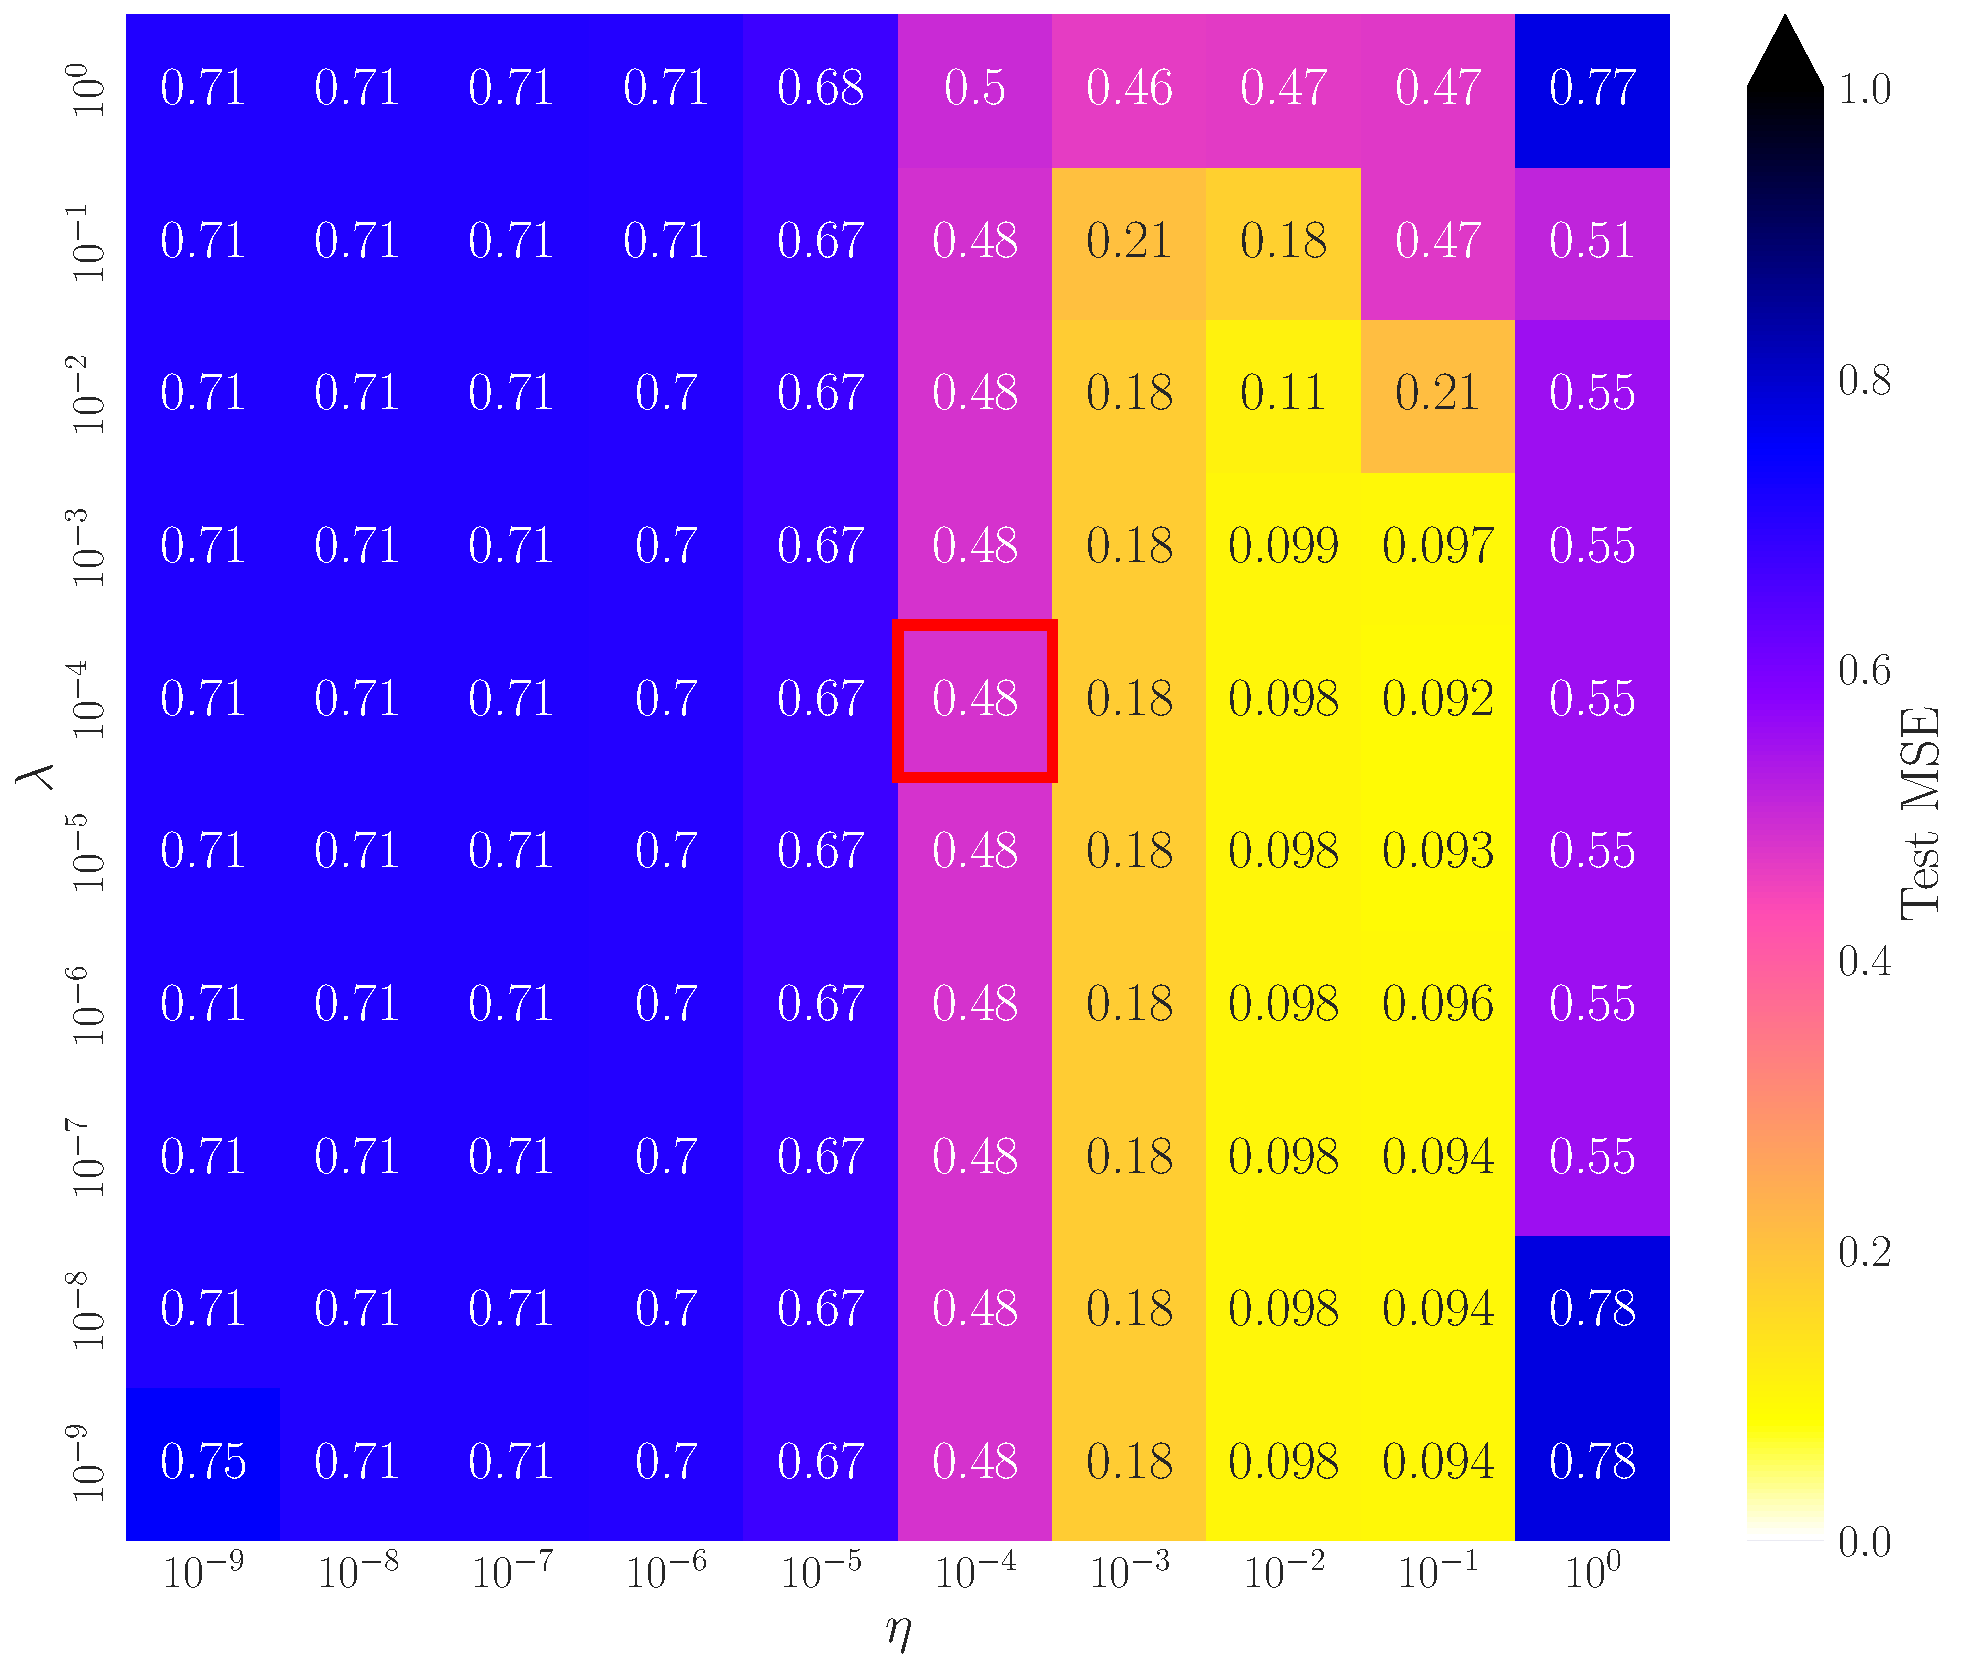
\includegraphics[width=\linewidth]{eta_lambda_analysis.pdf}
    \caption{Heatmap of the MSE as function of learning rate $\eta$ and regularisation parameter $\lambda$, using SGD with RMSProp as optimiser performing regression analysis of a 3 layered, 15-10-5 neurons, neural network. }
    \label{fig:reg_eta_lambda}
\end{figure}

\begin{figure}[h!]
    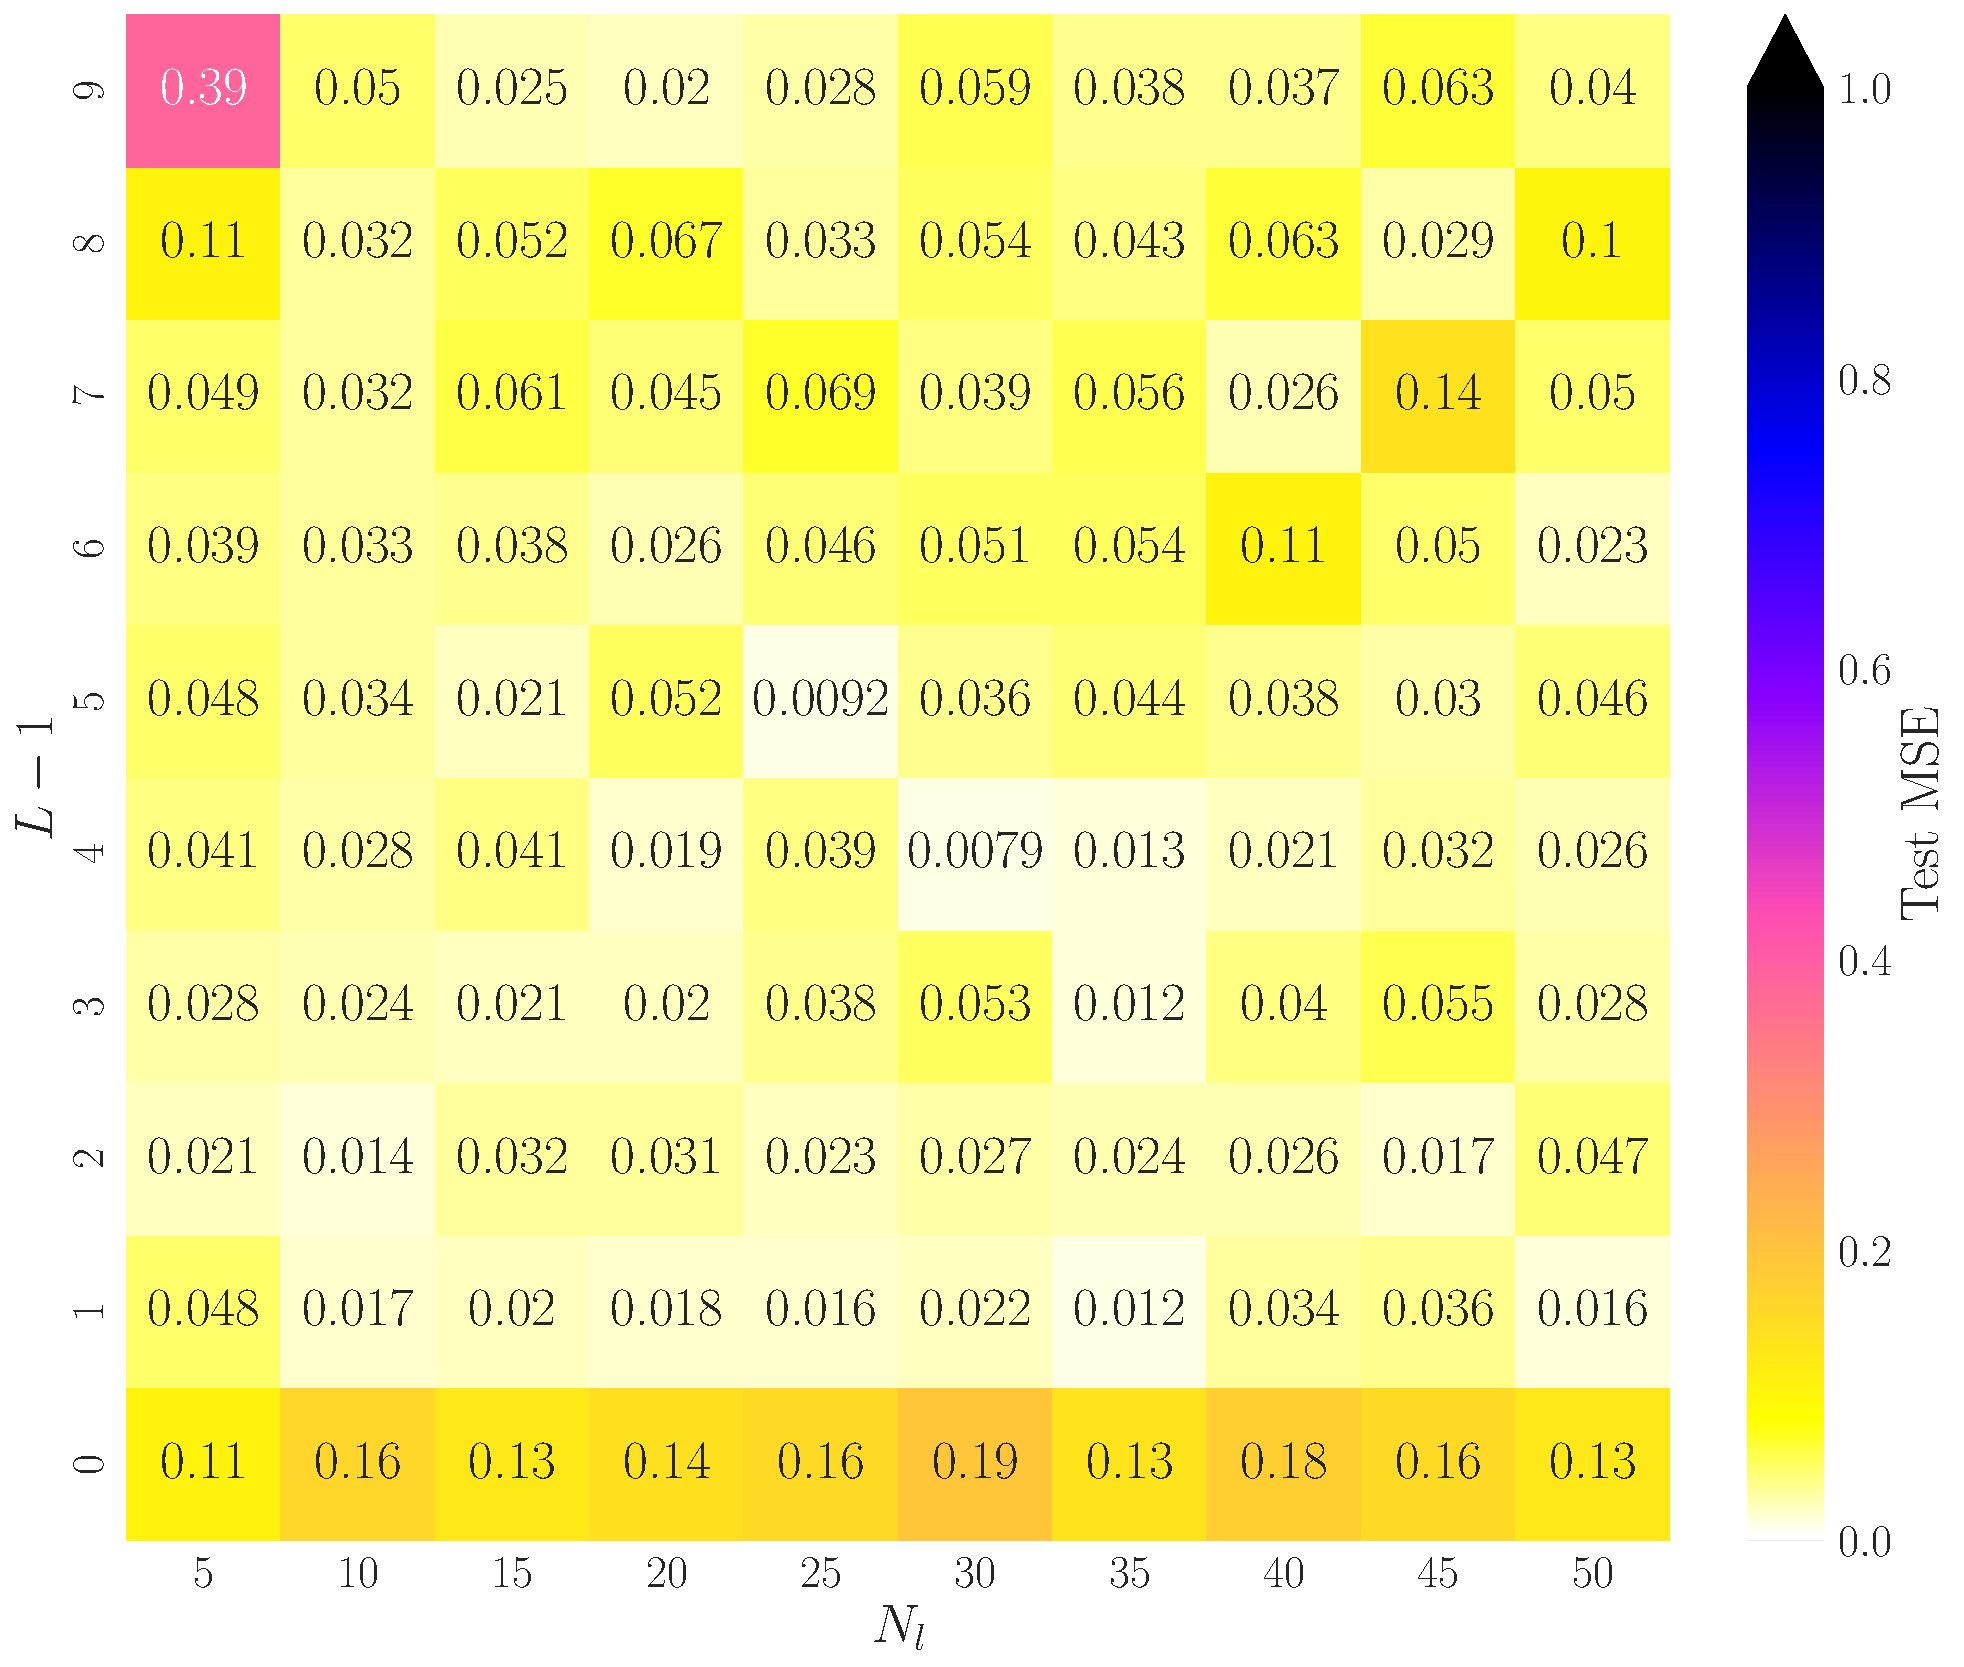
\includegraphics[width=\linewidth]{layer_neuron_analysis.pdf}
    \caption{Heatmap of the MSE as function of hidden layers $L-1$ and neurons per layer $N_l$, using SGD with RMSProp as optimiser performing regression analysis with $\eta=10^{-1}$ and $\lambda=10^{-4}$ }
    \label{fig:reg_layer_neuron}
\end{figure}

\begin{figure}[h!]
    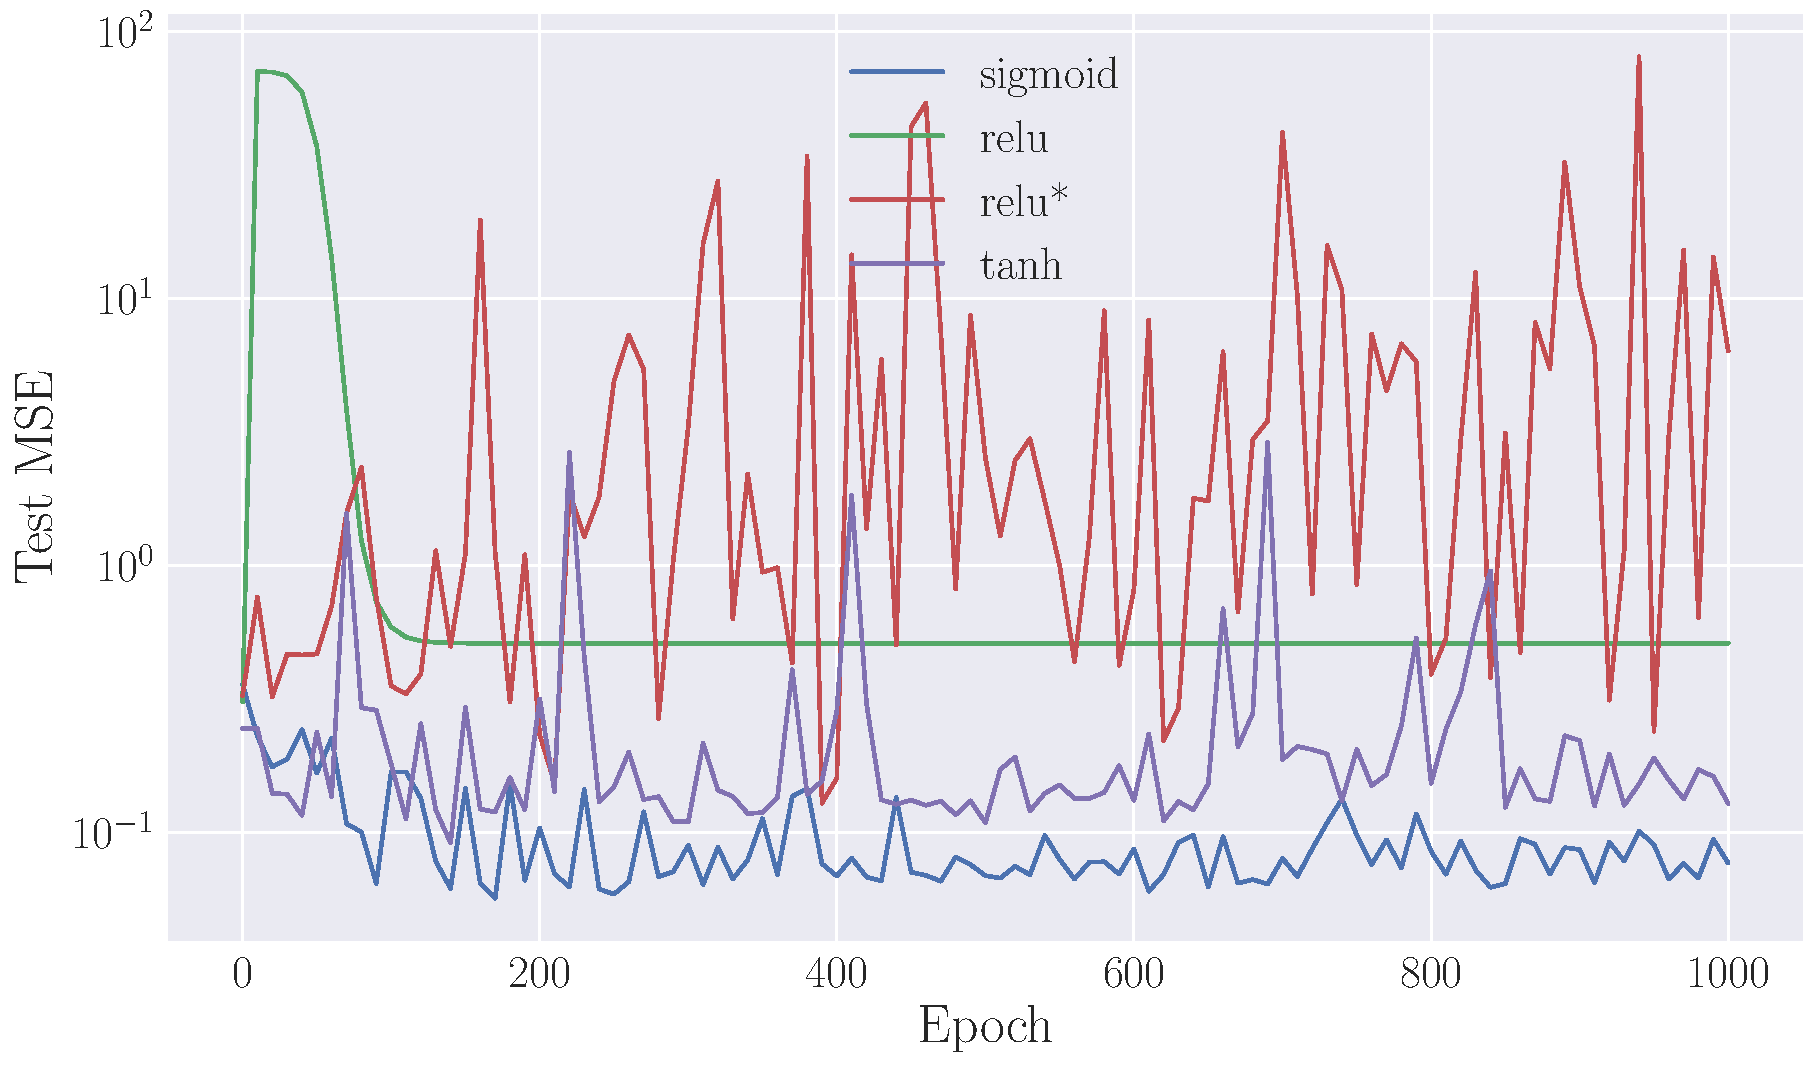
\includegraphics[width=\linewidth]{actFuncPer1000Epoch.pdf}
    \caption{Plot of the MSE for up to 1000 epochs, using SGD with RMSProp as optimiser performing regression analysis with $L-1=1$ hidden layer with $N_l=30$ neurons with $\eta=10^{-1}$ and $\lambda=10^{-4}$. The four different activation functions perform differently. Note the logarithmic MSE axis.}
    \label{fig:reg_act_epoch1000}
\end{figure}

\begin{figure}[h!]
    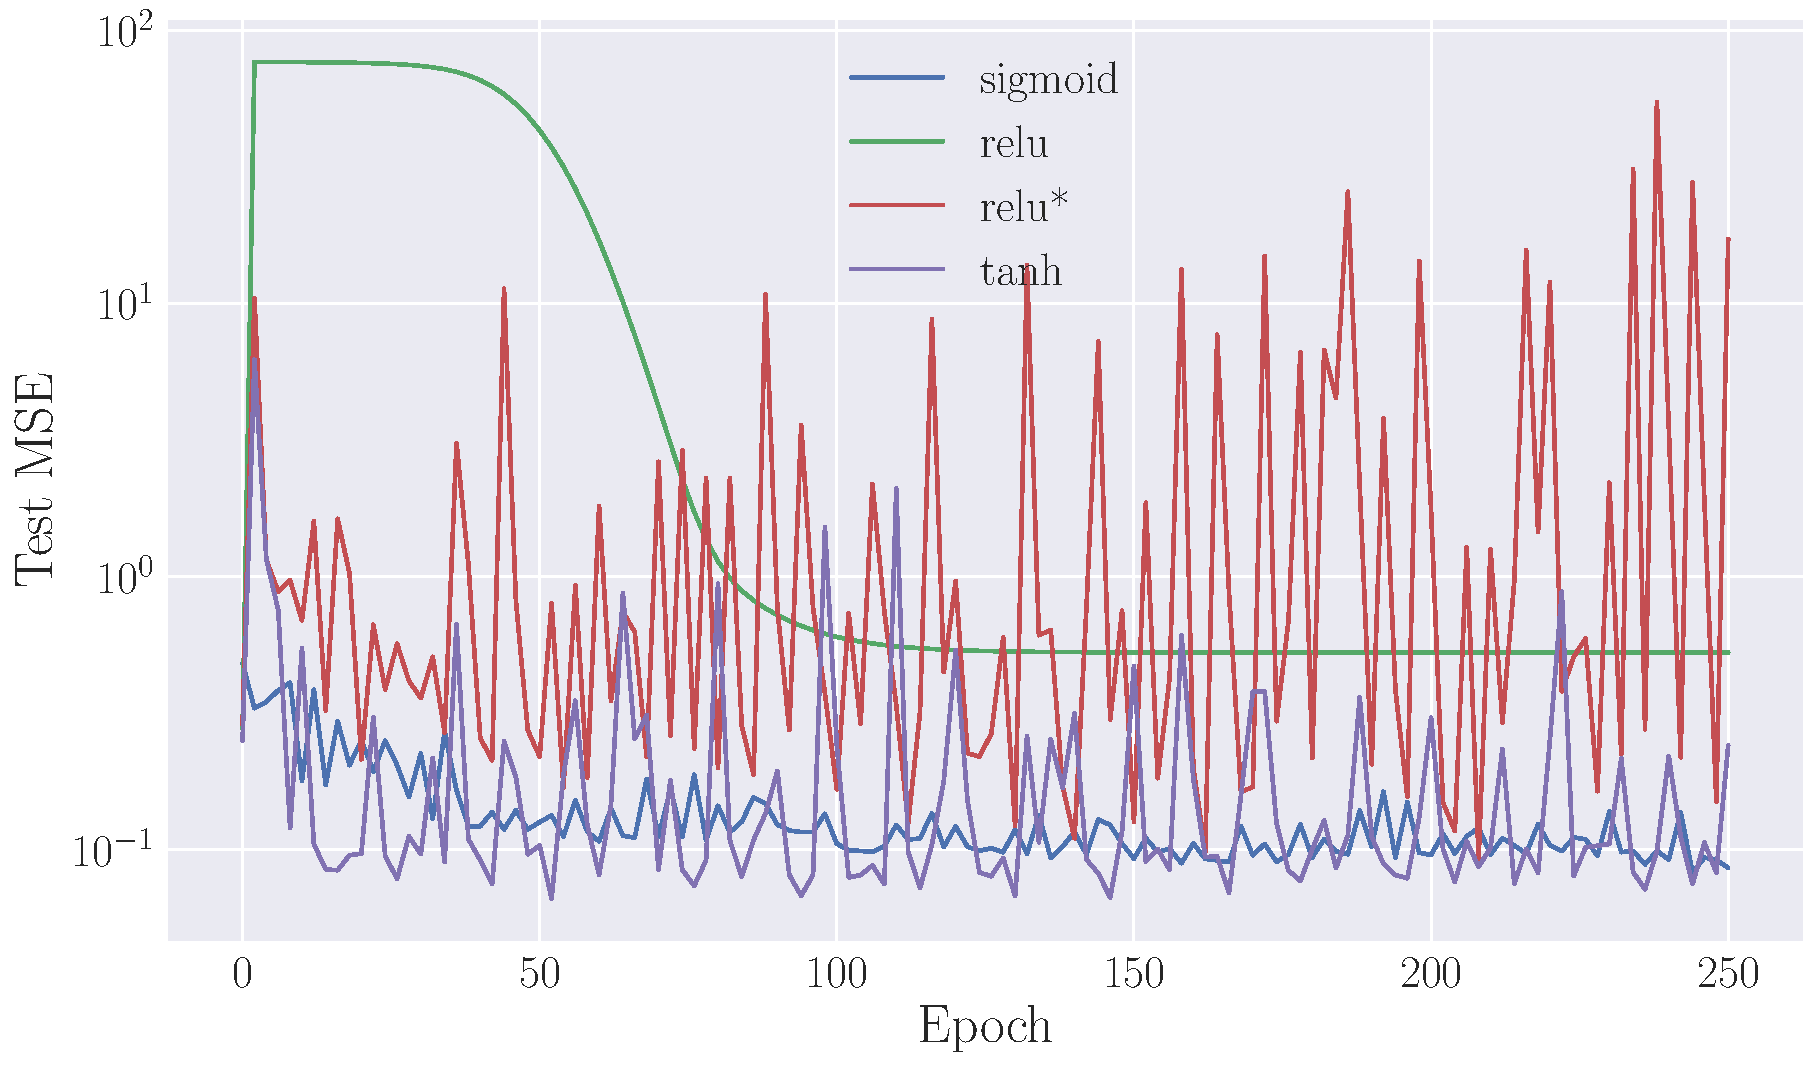
\includegraphics[width=\linewidth]{actFuncPerEpoch.pdf}
    \caption{Plot of the MSE for up to 250 epochs, using SGD with RMSProp as optimiser performing regression analysis with $L-1=1$ hidden layer with $N_l=30$ neurons with $\eta=10^{-1}$ and $\lambda=10^{-4}$. The four different activation functions perform differently. Note the logarithmic MSE axis.}
    \label{fig:reg_act_epoch}
\end{figure}

\begin{figure}[h!]
    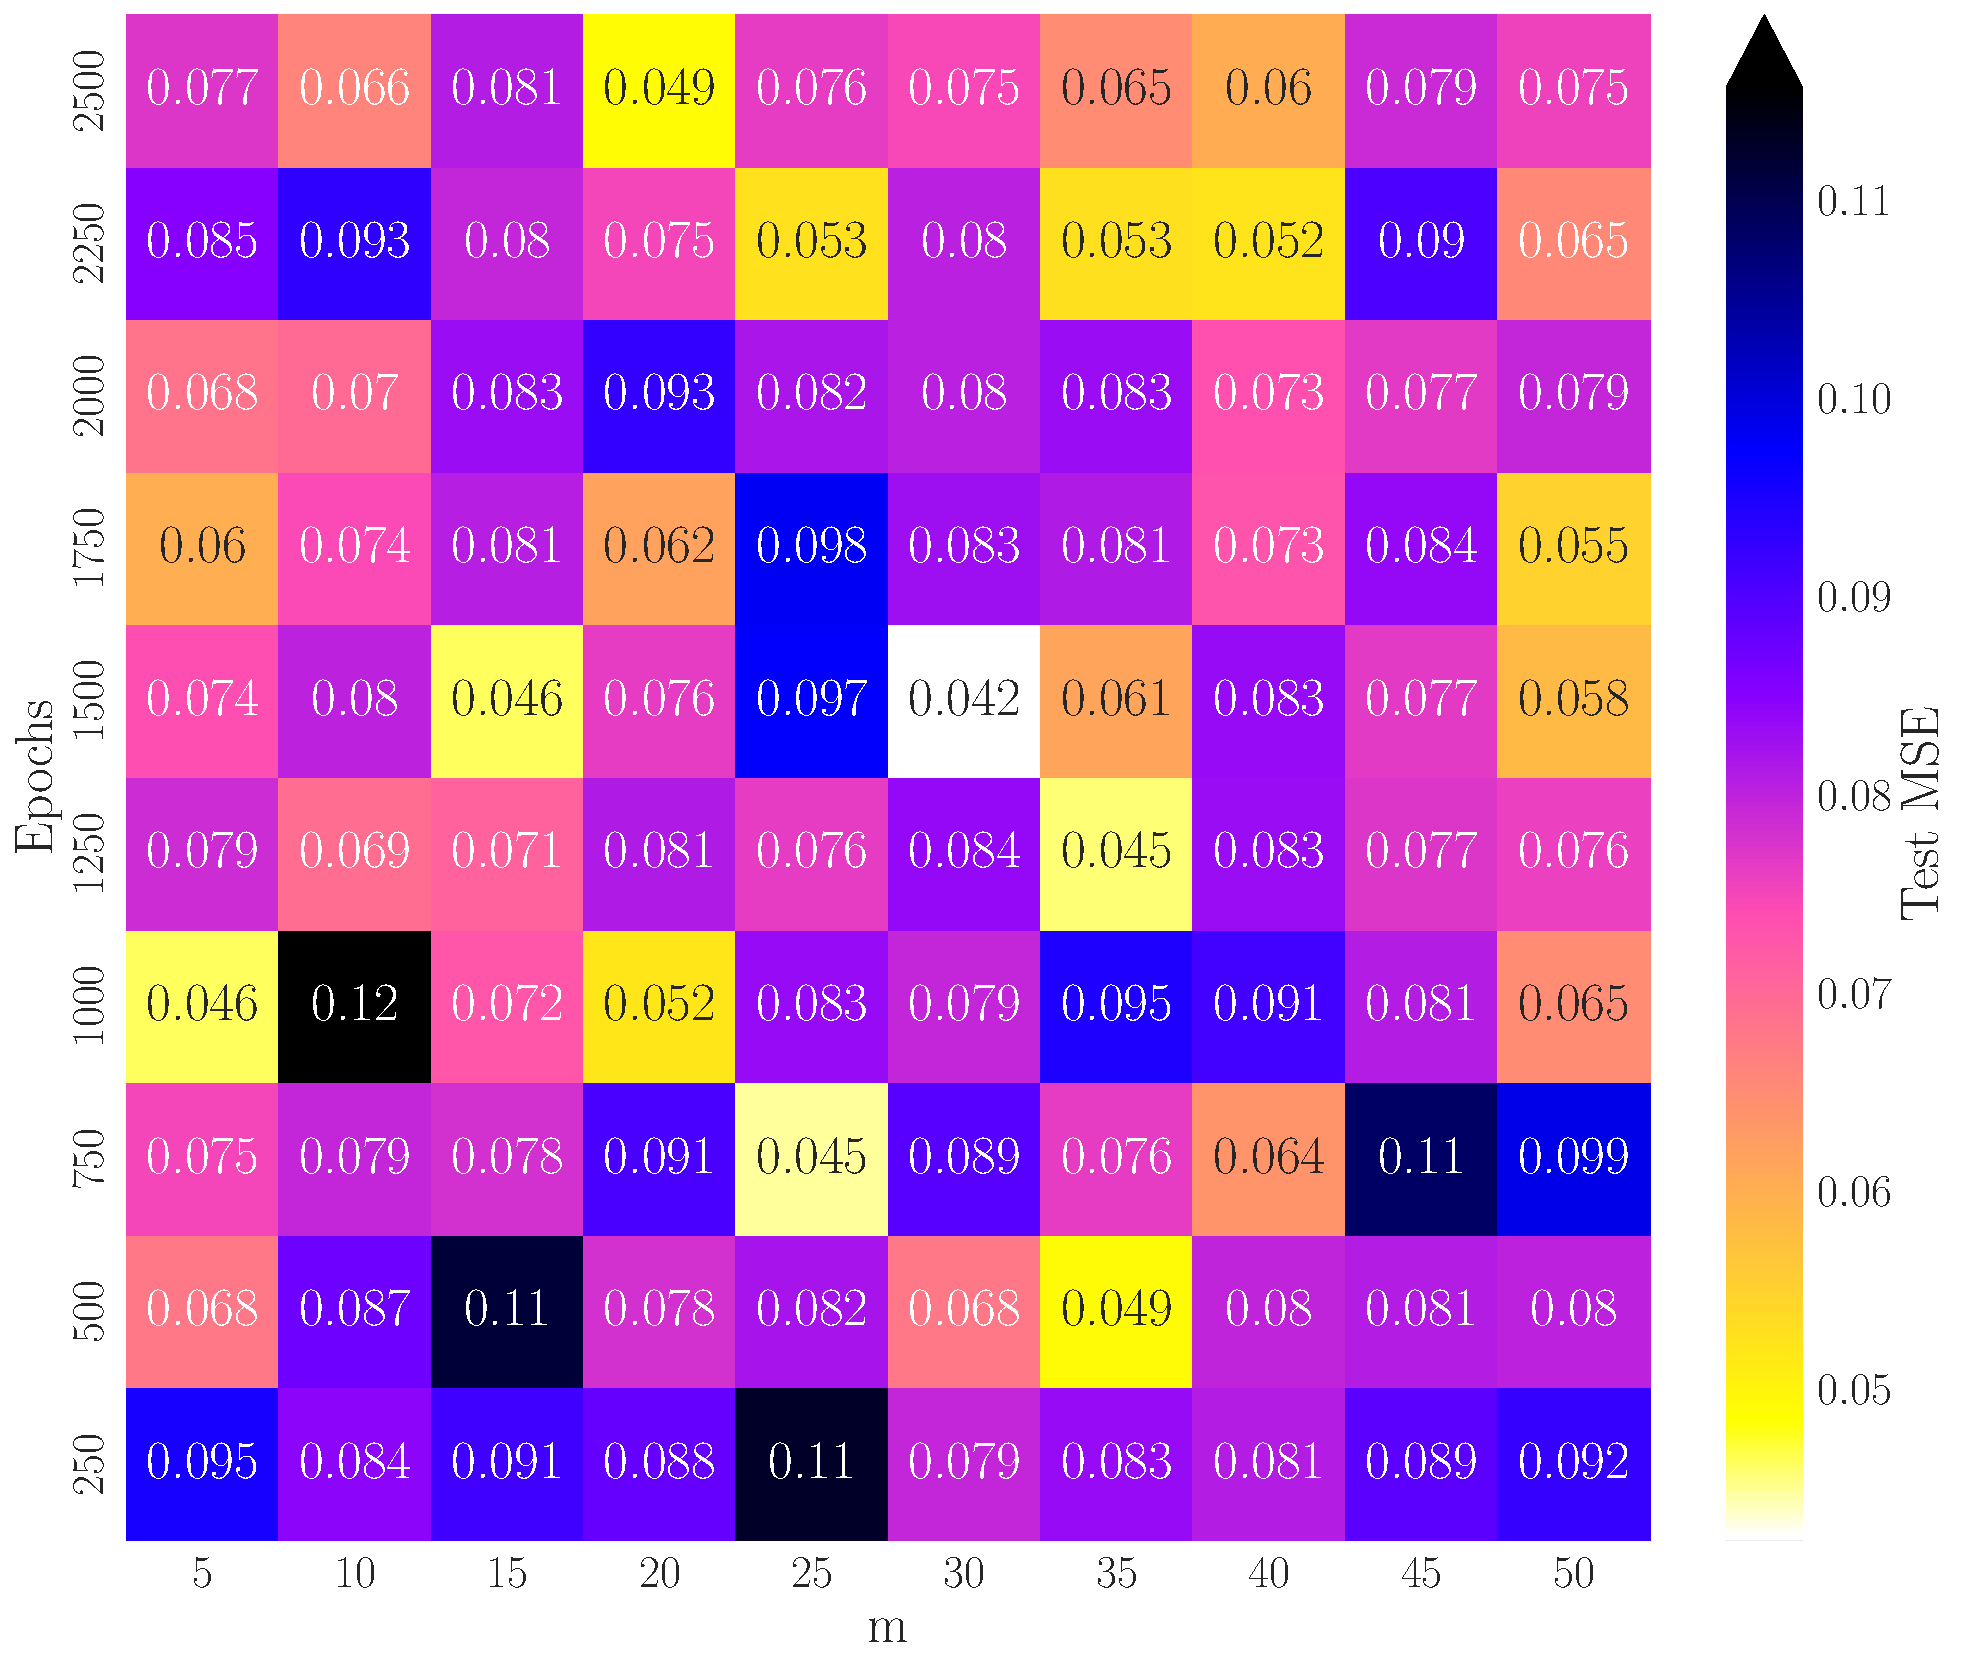
\includegraphics[width=\linewidth]{epoch_minibatch_analysis.pdf}
    \caption{Heatmap of the MSE as function of the number of minibatches $m$ and training epochs $N_l$, using SGD with RMSProp as optimiser performing regression analysis with $\eta=10^{-1}$ and $\lambda=10^{-4}$ }
    \label{fig:reg_minibatch_epoch}
\end{figure}

